
%version 2: \usepackage{hyperref}


%%%%%%%%%%%%%%%%%%%%%%%%%%%%%%%%%%%%%%%%%%%%%%%%%%%%%%%%%%%%%%%%%%%%%%%%
%Para las ecuaciones siempre es Ec.(n).
%Para las figuras siempre es Fig.n, incluso en el caption de la figura. Tambien las Tablas
%Para las referencias es [n]
%%%%%%%%%%%%%%%%%%%%%%%%%%%%%%%%%%%%%%%%%%%%%%%%%%%%%%%%%%%%%%%%%%%%%%%%

\documentclass[
reprint,
%notitlepage,
%superscriptaddress,
%groupedaddress,
%unsortedaddress,
%runinaddress,
%frontmatterverbose, 
%preprint,
%showpacs,preprintnumbers,
%nofootinbib,
%nobibnotes,
%bibnotes,
%11 pt,
amsmath,
amssymb,
%aps,
%pra,
prb,
%rmp,
%tightenlines %esto hizo el milagro de sacar los espacios en blancos estocásticos (?)
%prstab,
%prstper,
%floatfix,\textbf{}
]{revtex4-1} %Instalar primero para usarlo. Paquete malo.

%\documentclass[onecolumn, aps, amsmath,amssymb ]{article}
\usepackage{lipsum}  
\usepackage{graphicx}% Include figure files
\usepackage{subfig}
\usepackage{braket}
\usepackage{comment} %comment large chunks of text
\usepackage{dcolumn}% Align table columns on decimal point
\usepackage{bm}% bold math
%\usepackage{hyperref}% add hypertext capabilities
\usepackage[mathlines]{lineno}% Enable numbering of text and display math
%\linenumbers\relax % Commence numbering lines
\usepackage{mathtools} %% Para el supraíndice

\usepackage[nice]{nicefrac}

%%%%%%%El Señor Español%%%%%%%%%%%%%%%%%%%%%%%%%%%
\usepackage[utf8]{inputenc} %acento
\usepackage[
spanish, %El lenguaje.
es-tabla, %La tabla y no cuadro.
activeacute, %El acento.
es-nodecimaldot %Punto y no coma con separador de números
]{babel}
\usepackage{microtype} %para hacerlo más bonito :33 como vos (?) 
%%%%%%%%%%%%%%%%%%%%%%%%%%%%%%%%%%%%%%%%%%%%%%%%%%%
%%%%%%%%% Para que las imágenes se queden dónde las quiero (?
\usepackage{float}
%%%%%%%%%%
\usepackage{enumitem}
\usepackage{hyperref} % Para usar \url

%%%%%%%%Cambia a Fig de Figure%%%%%%%%%%
\makeatletter
\renewcommand{\fnum@figure}{Fig. \thefigure} 
\makeatother
%%%%%%%%%%%%%%%%%%%%%%%%%%%%%%%%%%%%%%%%
\raggedbottom


\begin{document}
%%%%%%%%%%%%%%%%%%%%%%%%%%%%%%%%%%Título%%%%%%%%%%%%%%%%%%%%%%%%%%%%%%%%%%%%%%
%%%%%%%%%%%%%%%%%%%%%%%%%%%%%%%%%%%%%%%%%%%%%%%%%%%%%%%%%%%%%%%%%%%%%%%%%%%%%%

\title{Práctica 0: Introducción a Python, Numpy, Matplotlib y Scipy.}
\author{Evelyn~G.~Coronel}

\affiliation{
Aprendizaje Profundo y Redes Neuronales Artificiales\\ Instituto Balseiro\\}

\date[]{\lowercase{\today}} %%lw para lw, [] sin date


\maketitle
%\onecolumngrid


\section*{Ejercicio 1}


\section*{Ejercicio 2}

\begin{figure}[H]
	\centering
	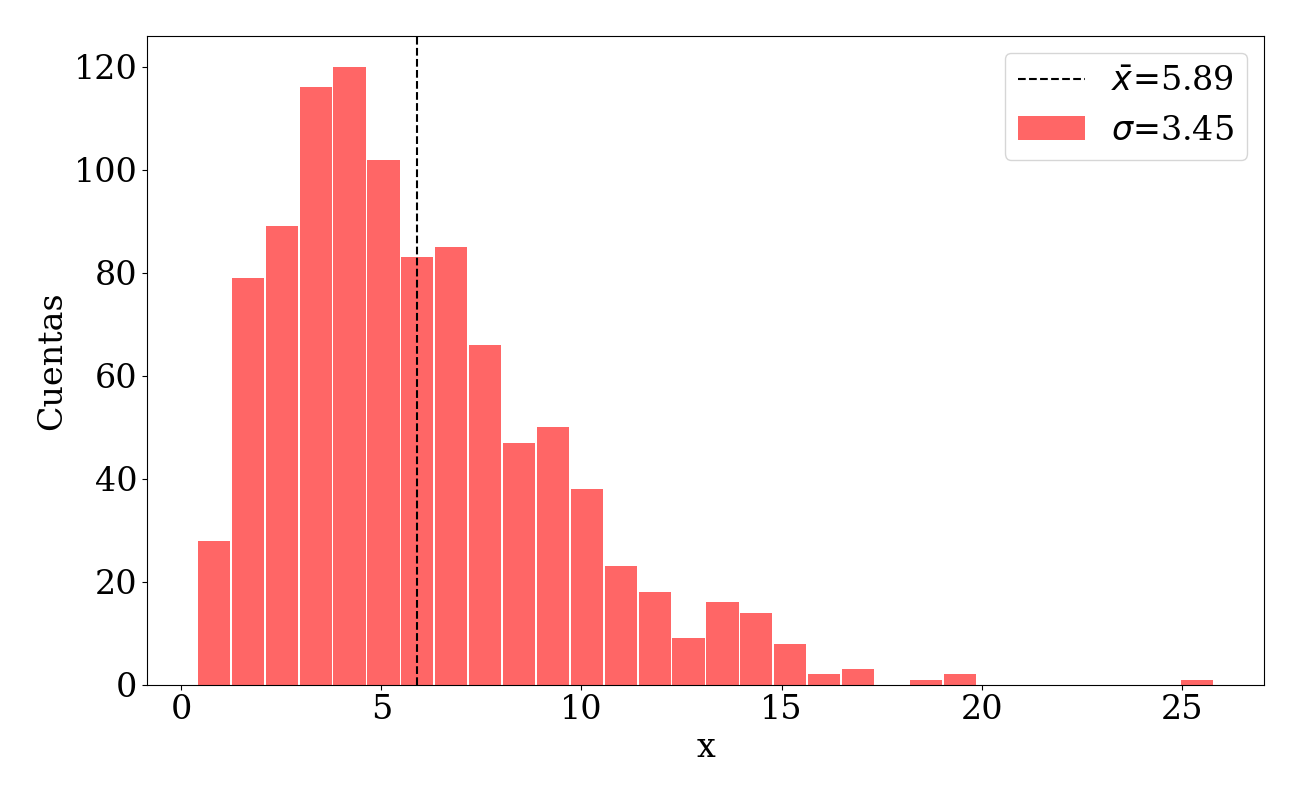
\includegraphics[width=0.5\textwidth]{ejer_2.png}
	\caption{Ejercicio 2}
	\label{fig:ejer2}
\end{figure}
	

\section*{Ejercicio 3}


\section*{Ejercicio 4}

\begin{figure}[H]
	\centering
	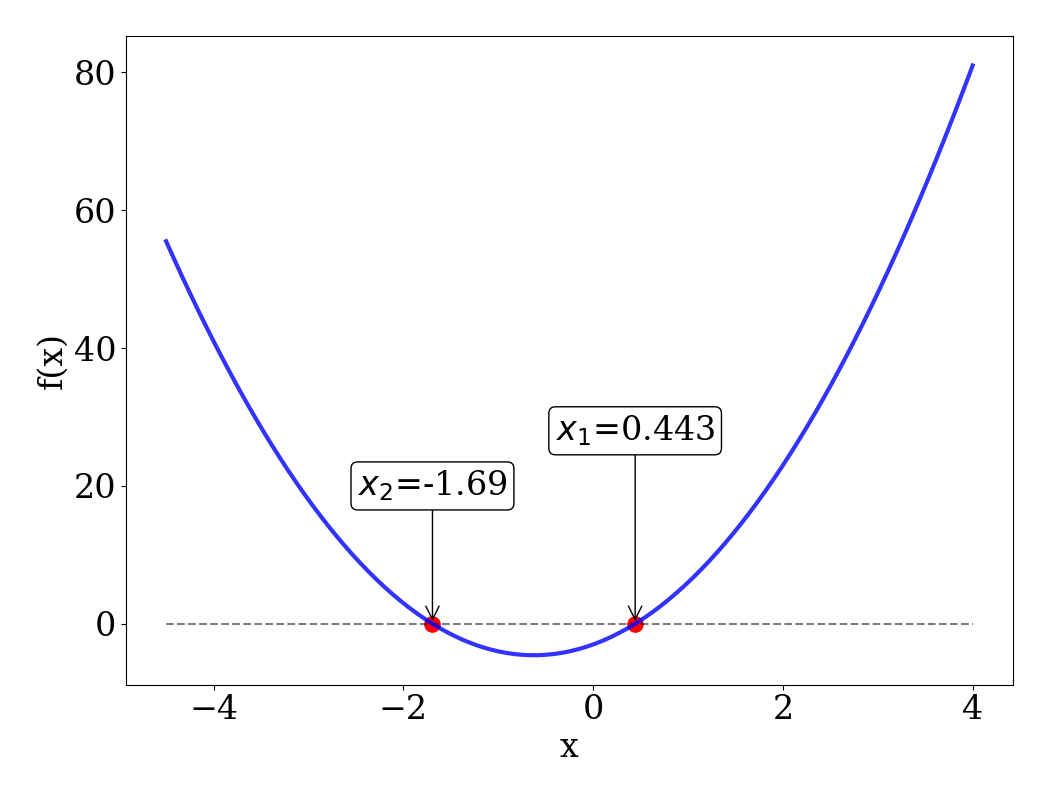
\includegraphics[width=0.5\textwidth]{ejer_4.png}
	\caption{Ejercicio 4}
	\label{fig:ejer4}
\end{figure}
	

\section*{Ejercicio 5}


\section*{Ejercicio 6}


\section*{Ejercicio 7}


\section*{Ejercicio 8}


\section*{Ejercicio 9}


\section*{Ejercicio 10}
\begin{figure}[H]
	\centering
	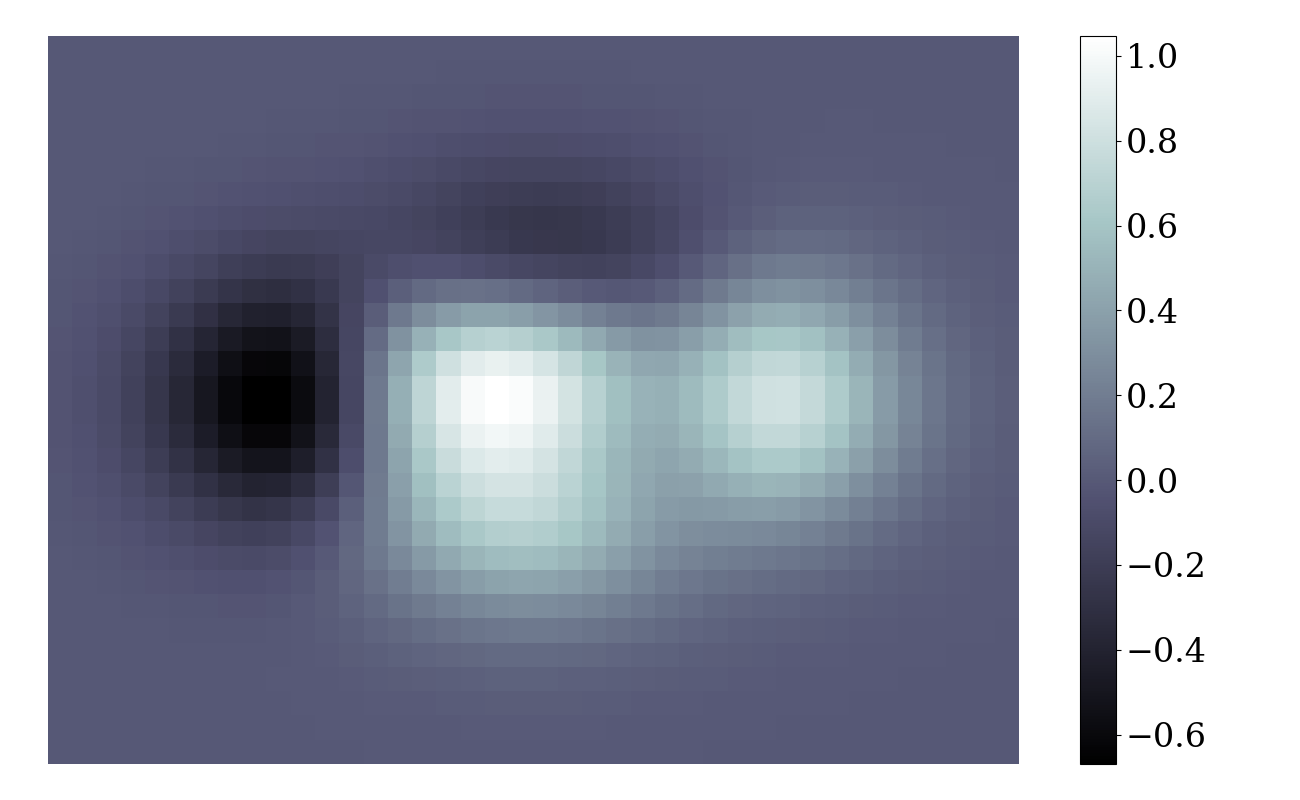
\includegraphics[width=0.5\textwidth]{ejer_10.png}
	\caption{Ejercicio 10}
	\label{fig:ejer10}
\end{figure}
	

\section*{Ejercicio 11}

\begin{figure}[H]
	\centering
	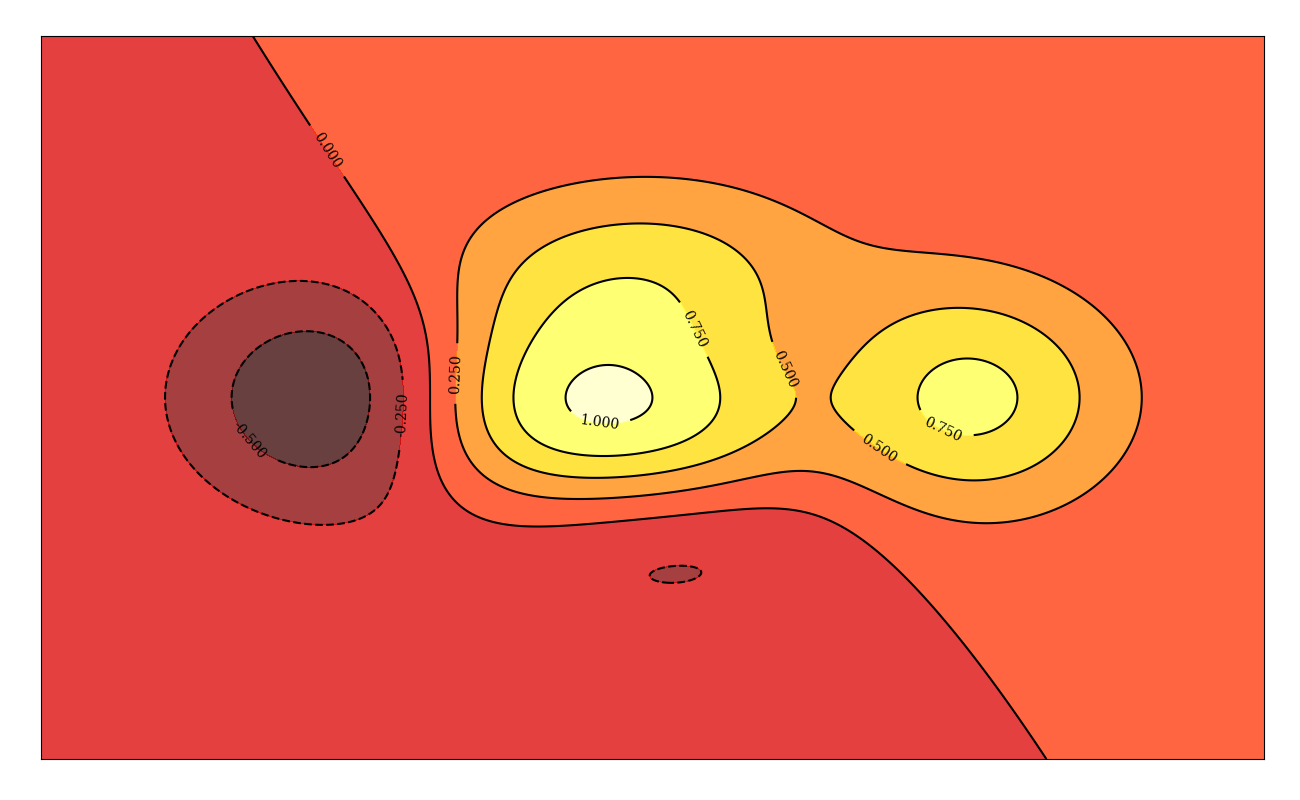
\includegraphics[width=0.5\textwidth]{ejer_11.png}
	\caption{Ejercicio 11}
	\label{fig:ejer11}
\end{figure}
	

\section*{Ejercicio 12}

\begin{figure}[H]
	\centering
	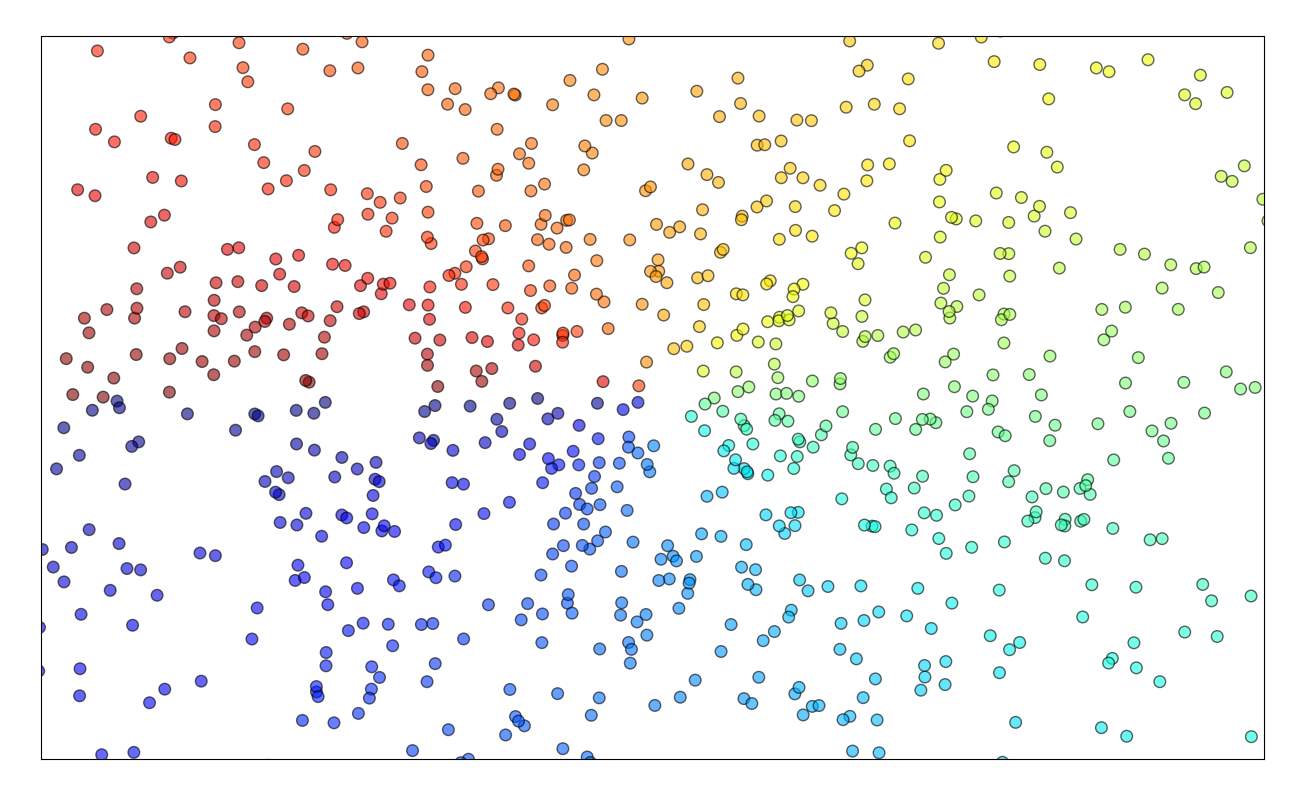
\includegraphics[width=0.5\textwidth]{ejer_12.png}
	\caption{Ejercicio 12}
	\label{fig:ejer12}
\end{figure}
	

\section*{Ejercicio 13: Movimiento del cardumen}

En este ejercicio se vió la utilidad de las clases en Python. Escribí una clase llamada "R2" que intenta describir un vector




\section*{Ejercicio 14}

\begin{figure}[H]
	\centering
	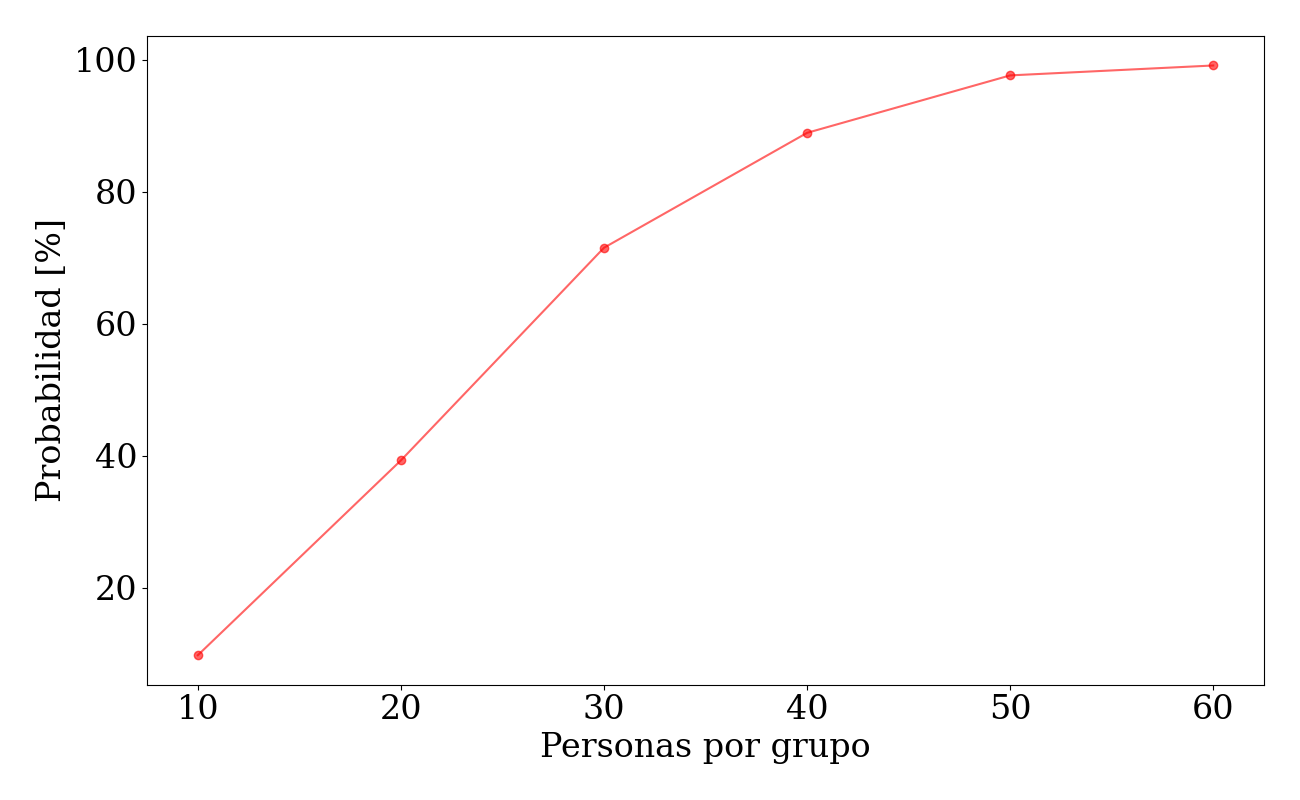
\includegraphics[width=0.5\textwidth]{ejer_14.png}
	\caption{Ejercicio 14}
	\label{fig:ejer14}
\end{figure}
	

\section*{Ejercicio 15}

\begin{figure}[H]
	\centering
	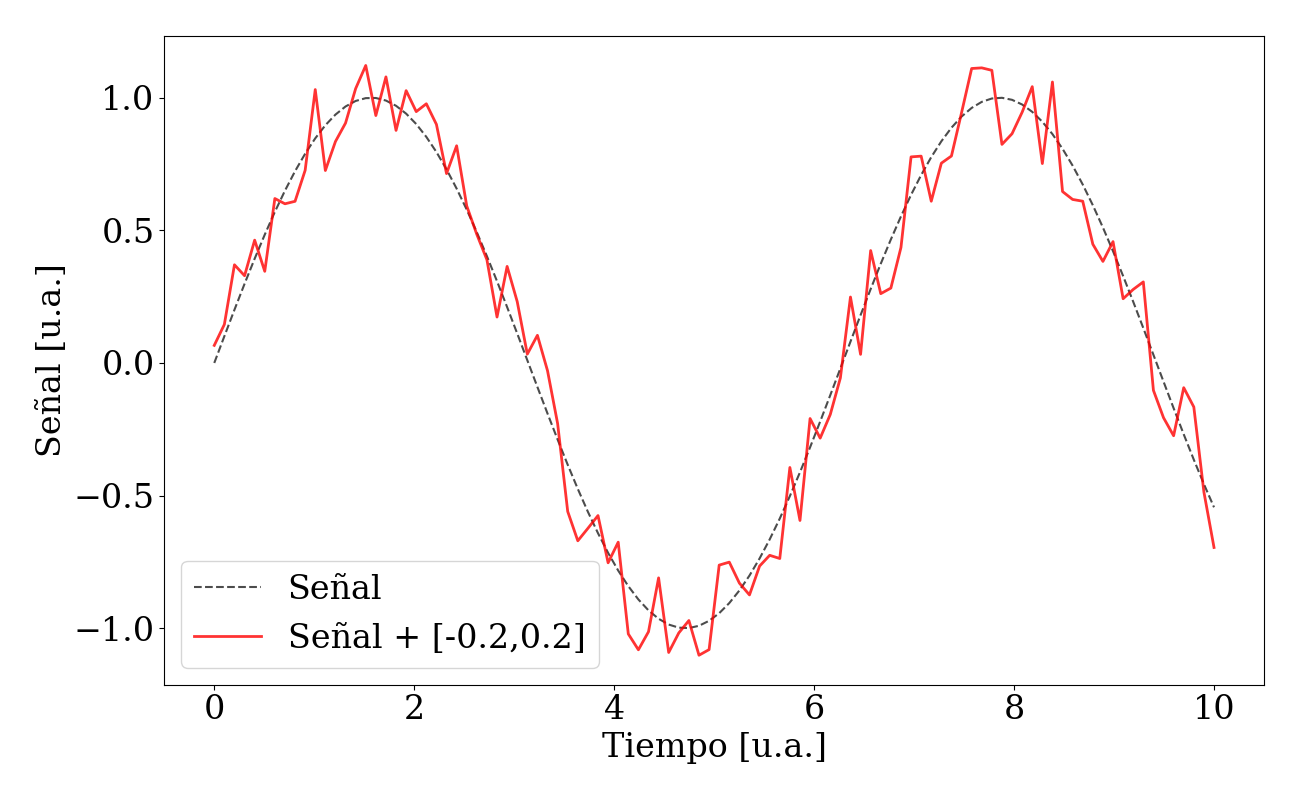
\includegraphics[width=0.5\textwidth]{ejer_15.png}
	\caption{Ejercicio 15}
	\label{fig:ejer15}
\end{figure}
	

\end{document}